\chapter{\chatextformulaSelection}\label{cha:formulaSelection}

In this chapter we will investigate efficient schemes to represent collections of formulas with similar structure in one tensor network.

% Relational encoding of the selection map
\begin{definition}
	Given a set of $\seldim$ formulas $\{\formulaof{\selindex} : \selindexin\}$, we define the formula selecting map as
		\[  \fselectionmapat{\shortcatvariables,\selvariable} : \atomstates \times [\seldim] \rightarrow [2] \]
	defined for $\selindexin$ by
		\[ \fselectionmapat{\shortcatvariables=\atomindices,\selvariable=\selindex} =  \formulaofat{\selindex}{\shortcatvariables=\atomindices} \, . \]
\end{definition}

% Selection Variables
We introduce a selection variable $\selvariable$ and depict the formula selection in Figure~\ref{fig:formulaSelectionMap}.

% Depiction
\begin{figure}[h]
\begin{center}
	\begin{tikzpicture}[scale=0.35, thick] % , baseline = -3.5pt

    \begin{scope}
        [shift={(-20,0)}]
        \node[anchor=center] (text) at (-1,3) {${a)}$};

        \node [circle, draw, thick, fill=gray!50, minimum size = \nodeminsize] (T1) at (0,0) {\tiny $\catvariableof{0}$};
        \node [circle, draw, thick, fill=gray!50, minimum size = \nodeminsize] (T2) at (3,0) {\tiny $\catvariableof{1}$};
        \node[anchor=center] (text) at (6,0) {${\cdots}$};
        \node [circle, draw, thick, fill=gray!50, minimum size = \nodeminsize] (T3) at (9,0) {};
        \node[anchor=center] (text) at (9,0) {\tiny $\catvariableof{\seldim\shortminus1}$};

        \node [circle, draw, thick, fill=gray!50, minimum size = \nodeminsize] (T4) at (12,3) {};
        \node[anchor=center] (text) at (12,3) {\tiny $\selvariable$};

        \draw[->-] (6,3) -- (6,6);

        \node [circle, draw, thick, fill=gray!50, minimum size = \nodeminsize] (S) at (6,6) {};
        \node[anchor=center] (text) at (6,6) {\tiny $\headvariableof{\fselectionmap}$};

        \draw[->-] (T1) -- (6,3);
        \draw[->-] (T2) -- (6,3);
        \draw[->-] (T3) -- (6,3);
        \draw[->-] (T4) -- (6,3);

    \end{scope}


    \node[anchor=center] (text) at (-1,3) {${b)}$};


    \begin{scope}
        [shift={(0,-2)}]
        \draw[-<-] (0,1)--(0,-1) node[midway,left] {\tiny $\catvariableof{0}$};
        \draw[-<-] (1.5,1)--(1.5,-1) node[midway,left] {\tiny $\catvariableof{1}$};
        \node[anchor=center] (text) at (3,0) {$\cdots$};
        \draw[-<-] (4,1)--(4,-1) node[midway,right] {\tiny $\catvariableof{\seldim\shortminus1}$};
    \end{scope}

    \draw (-1,1) rectangle (5,-1);
    \node[anchor=center] (text) at (2,0) {$\bencodingof{\fselectionmap}$};
    \draw[->-] (2,1) -- (2,3) node[midway, right]  {\tiny $\headvariableof{\fselectionmap}$};
    \draw[-<-] (5,0) -- (7,0) node[midway, above] {\tiny $\selvariable$};


\end{tikzpicture}
\end{center}
\caption{Representation of the Formula Selecting map as a 
a) Graphical Model with a selection variable $\fselectionmap$.
b) Dual Tensor Core with selection variable corresponding with an additional axis.}
\label{fig:formulaSelectionMap}
\end{figure}


% Decomposition
A naive representation of the formula selecting map is as a sum
	\[ \fselectionmap = \sum_{\selindexin} \formulaofat{\selindex}{\shortcatvariables}  \otimes \onehotmapofat{\selindex}{\selvariable} \, . \]
Such a representation scheme requires linear resources in the number of formulas.
We will show in the following, that we can exploit common structure in formulas to drastically reduce this resource consumption.



\sect{Construction schemes}

% Naturality of folding
Let us now investigate efficient schemes to define sets of formulas to be used in the definition of $\fselectionmap$.
We will motivate the folding of the selection variable into multiple selection variables by compositions of selection maps.


\subsect{Connective Selecting Tensors}

We represent choices over connectives with a fixed number of arguments by adding a selection variable to the cores and defining each slice by a candidate connective.

% Formal map
\begin{definition}\label{def:connectiveSelector}
	Let $\{\connectiveof{0},\ldots,\connectiveof{\seldimof{\cselectionsymbol}-1}\}$ be a set of connectives with $\atomorder$ arguments.
	The associated connective selection map is
		\[ \cselectionmapat{\shortcatvariables,\selvariableof{\cselectionsymbol}}
		: \atomstates \times [\seldimof{\cselectionsymbol}] \rightarrow [2] \]
	defined for each $\selindexofin{\cselectionsymbol}$ and $\shortcatindices\in\atomstates$ by 
		\[ \cselectionmapat{\shortcatvariables=\shortcatindices,\indexedselvariableof{\cselectionsymbol}} 
		= \connectiveofat{\selindexof{\cselectionsymbol}}{\shortcatvariables=\shortcatindices}  \, . \]
\end{definition}

We depict the relational encoding of connective selection maps in Figure~\ref{fig:connectiveSelector}.

\begin{figure}[h]
\begin{center}
	\begin{tikzpicture}[scale=0.35, thick] % , baseline = -3.5pt

\begin{scope}[shift={(-20,0)}]
	\node[anchor=center] (text) at (-1,3) {${a)}$};

	\node [circle, draw, thick, fill=gray!50, minimum size = \nodeminsize] (T1) at (0,0) {\tiny $\catvariableof{0}$};
	\node [circle, draw, thick, fill=gray!50, minimum size = \nodeminsize] (T2) at (3,0) {\tiny $\catvariableof{1}$};
	\node[anchor=center] (text) at (6,0) {${\cdots}$};
	\node [circle, draw, thick, fill=gray!50, minimum size = \nodeminsize] (T3) at (9,0) {};
	\node[anchor=center] (text) at (9,0) {\tiny $\catvariableof{\atomorder\shortminus1}$};
	
	\node [circle, draw, thick, fill=gray!50, minimum size = \nodeminsize] (T4) at (12,0) {};
	\node[anchor=center] (text) at (12,0) {\tiny $\cselinputvariable$};

	
	\node [circle, draw, thick, fill=gray!50, minimum size = \nodeminsize] (S2) at (6,4.5) {};
	\node[anchor=center] (text) at (6,4.5) {\tiny $\catvariableof{\cselectionsymbol}$};
	
	\coordinate (S) at (6,2.5);
	\draw[->] (S) -- (S2);

	\draw[->] (T1) -- (S);
	\draw[->] (T2) -- (S);
	\draw[->] (T3) -- (S);
	\draw[->] (T4) -- (S);
	
\end{scope}


\node[anchor=center] (text) at (-1,3) {${b)}$};
	
	
\begin{scope}[shift={(5,2)}]

	\begin{scope}[shift={(0,-2)}]
		\draw[<-] (0,1)--(0,-1) node[midway,left] {\tiny $\catvariableof{0}$}; 
		\draw[<-] (1.5,1)--(1.5,-1) node[midway,left] {\tiny $\catvariableof{1}$}; 
		\node[anchor=center] (text) at (3,0) {$\cdots$};
		\draw[<-] (4,1)--(4,-1) node[midway,right] {\tiny $\catvariableof{\atomorder\shortminus1}$}; 
	\end{scope}
	
\draw (-1,1) rectangle (5,-1);
\node[anchor=center] (text) at (2,0) {$\bencodingof{\cselectionmap}$};
\draw[->] (2,1) -- (2,3) node[midway, right]  {\tiny $\catvariableof{\cselectionsymbol}$};
\draw[<-] (5,0) -- (7,0) node[midway, above] {\tiny $\cselinputvariable$};

\end{scope}
	

\end{tikzpicture}
\end{center}
\caption{Connective Selector.}
\label{fig:connectiveSelector}
\end{figure}

%Following a different perspective: skeleton+atomindices at atomic expression level, atomindices at complex expression level!
%Having an parametrization of binary connectives by $\circ_{\selindex}$ we can define the corresponding connective selector tensor by
%	\[ \rencodingof{\circ}_{\selindex,:,:} = \rencodingof{\circ_{\selindex}}_{:,:} \, . \]

\begin{remark}[$\htformat$ Interpretation of Superposed Formula Tensor Networks]\label{rem:HTDecomSFT}
	Continuing Remark ~\ref{rem:HTDecomFT}: 
	Superposed Formula Tensors have a decomposition into a $\htformat$ as sketched here, where we distinguish between formula selection subspaces (indices $\selindexof{\selenumerator}$) and atomic subspaces (indices $\atomlegindexof{\atomenumerator})$.
	At each formula selection we thus have a decomposition into three subspaces, two of atomic formulas and one for the formula selection.
\end{remark}




\subsect{Variable Selecting Tensor Network}

%\red{Works also for categorical variables! -> Into Contraction Calculus?}

%% Definition
\begin{definition}\label{def:variableSelector}
	The selection of one out of $\seldim$ variables in a list $\catvariableof{[\seldim]}$ is done by variable selecting maps
	\begin{align}
		\vselectionmapat{\catvariableof{[\seldim]},\selvariableof{\vselectionsymbol}}:  \left(\bigtimes_{\selindex\in[\seldim]}[2]\right) \times [\seldim]  \rightarrow [2]
	\end{align}
	are defined coordinatewise by
	\begin{align}
		\vselectionmapat{\indexedcatvariableof{0},\ldots,\indexedcatvariableof{\seldim-1},\indexedselvariableof{\vselectionsymbol}} = \catindexof{\selindex} \, .
	\end{align}
\end{definition}
	
% Interpretation as multiplex gate
Variable selecting maps appear in the literature as multiplex gates (see Definition 5.3 in \cite{koller_probabilistic_2009}).

The relational encoding of the variable selection map has a decomposition 
\begin{align*}
	\rencodingofat{\vselectionmap}{\vselectionheadvar,\catvariableof{[\seldimof{\vselectionsymbol}]}}
	= \sum_{\selindexofin{\vselectionsymbol}} 
	\rencodingofat{\atomicformulaof{\selindexof{\vselectionsymbol}}}{\vselectionheadvar,\catvariableof{\selindexof{\vselectionsymbol}}} \otimes  \onehotmapofat{\selindexof{\vselectionsymbol}}{\selvariableof{\vselectionsymbol}} \, . 
\end{align*}
This structure is exploited in the next theorem to derive a tensor network decomposition of $\rencodingof{\vselectionmap}$.

\begin{theorem}[Decomposition of Variable Selecting Maps]\label{the:varSelectorDecomposition}
	Given a list $\catvariableof{[\seldimof{\vselectionsymbol}]}$ of variables, we define for each $\selindexofin{\vselectionsymbol}$ the tensors
		\[ \selectorcomponentofat{\selindexof{\vselectionsymbol}}{\catvariableof{\selindexof{\vselectionsymbol}},\selvariableof{\vselectionsymbol}} 
		= \identityat{\vselectionheadvar,\catvariableof{\selindexof{\vselectionsymbol}}} \otimes \onehotmapofat{\selindexof{\vselectionsymbol}}{\selvariableof{\vselectionsymbol}} 
		+ \onesat{\vselectionheadvar,\catvariableof{\selindexof{\vselectionsymbol}}} \otimes \left(\onesat{\selvariableof{\vselectionsymbol}} - \onehotmapofat{\selindexof{\vselectionsymbol}}{\selvariableof{\vselectionsymbol}} \right) \, . 
		\]
	Then we have (see Figure~\ref{fig:SelectorDecomposition})
		\[ \rencodingofat{\vselectionmap}{\vselectionheadvar,\catvariableof{[\seldim]},\selvariableof{\vselectionsymbol}}
		= \contractionof{
			\{\selectorcomponentofat{\selindexof{\vselectionsymbol}}{\vselectionheadvar,\catvariableof{\selindexof{\vselectionsymbol}},\selvariableof{\vselectionsymbol}} \, : \, \selindexofin{\vselectionsymbol}\}
		}{\vselectionheadvar,\catvariableof{[\seldim]},\selvariableof{\vselectionsymbol}} \, .
		\]
\end{theorem}
\begin{proof}
	We show the equivalence of the tensors on an arbitrary coordinates.
	For $\tilde{\selindex}_{\vselectionsymbol}\in[\seldimof{\vselectionsymbol}]$, $\vselectionheadvar\in[2]$ and $\catindexof{[\seldimof{\vselectionsymbol}]}\in\bigtimes_{\catenumerator\in[\seldimof{\vselectionsymbol}]}[2]$ we have
	\begin{align*}
		& \contractionof{
			\{\selectorcomponentofat{\selindexof{\vselectionsymbol}}{\vselectionheadvar,\catvariableof{\selindexof{\vselectionsymbol}},\selvariableof{\vselectionsymbol}} \, : \, \selindexofin{\vselectionsymbol}\}
		}{\indexedheadvariableof{\vselectionsymbol},\indexedcatvariableof{[\seldim]},\selvariableof{\vselectionsymbol} = \tilde{\selindex}_{\vselectionsymbol}} \\
		& \quad = 
		\prod_{\selindexofin{\vselectionsymbol}} \selectorcomponentofat{\selindexof{\vselectionsymbol}}{
			\indexedheadvariableof{\vselectionsymbol},\indexedcatvariableof{\selindexof{\vselectionsymbol}},\selvariableof{\vselectionsymbol}=\tilde{\selindex}_{\vselectionsymbol}
			} \\
		& \quad = \selectorcomponentofat{\tilde{\selindex}_{\vselectionsymbol}}{
			\indexedheadvariableof{\vselectionsymbol},\indexedcatvariableof{\selindexof{\vselectionsymbol}},\selvariableof{\vselectionsymbol}=\tilde{\selindex}_{\vselectionsymbol}
		} \\
		& \quad = 
		\begin{cases}
		 	1 & \text{if} \quad \headindexof{\vselectionsymbol} = \catindexof{\selindexof{\vselectionsymbol}} \\
		 	0 & \text{else}  
		 \end{cases} \\ 
		 & = \rencodingofat{\vselectionmap}{\indexedheadvariableof{\vselectionsymbol},\indexedcatvariableof{[\seldim]},\selvariableof{\vselectionsymbol}=\tilde{\selindex}_{\vselectionsymbol}}
	\end{align*}
	In the second equality, we used that the tensor $\selectorcomponentof{\selindexof{\vselectionsymbol}}$ have coordinates $1$ whenever $\tilde{\selindex}_{\vselectionsymbol}\neq\selindexof{\vselectionsymbol}$.
\end{proof}


The decomposition provided by \theref{the:varSelectorDecomposition} is in a CP format, as will be further discussed in \charef{cha:sparseCalculus}.
The introduced tensors $\selectorcomponentof{\selindexof{\vselectionsymbol}}$ are Boolean, but not directed and therefore encodings of relations but not functions (see \charef{cha:basisCalculus}).

%%% Decomposition
%% ! THIS IS NOT \theref{the:functionDecompositionBasisCP}, but works on slice sparsity!

%Using that the encoding $\rencodingof{\atomicformulaof{\selindex}}$ of atomic formulas admits and elementary decomposition (see \theref{the:AtomicFTensor}) we notice that Equation~\ref{eq:selectorDecomposition} describes a so-called monomial decomposition, which will be introduced in \defref{def:polynomialSparsity}.
%We can apply \theref{the:sliceToCP} to find a decomposition of $\selectorcore$ in a CP format consisting of cores
%\begin{align}
%	\selectorcoreof{\selindex} = \dirdeltaof{\randomxof{\selindex},\selvariable} \otimes \onehotmapof{\selindex}
%	+ \sum_{\tilde{\selindex}\in[\seldim] \, , \, \tilde{\selindex}\neq\selindex} \onesof{\randomxof{\selindex},\selvariable} \otimes \onehotmapof{\tilde{\selindex}} \, .
%\end{align}	
%The CP decomposition is depicted in Figure~\ref{fig:SelectorDecomposition}.
%
%% Selectorcores are non-functional relational encodings
%We notice, that the selector cores $\selectorcoreof{\selindex}$ are encodings of a relation, which is not a function.
%Therefore, they are binary but not directed tensors.
%Their contraction 
%\begin{align}\label{eq:selectorDecomposition}
% 	\selectorcore = 
%	\contractionof{\{\selectorcomponentof{\selindex}\, : \, \selindexin\}}
%	{\{\randomxof{0},\ldots,\randomxof{\seldim-1},\selvariable\}}
%\end{align}
%is the relational encoding of the function $\vselectionmap$ and thus binary and directed.


%% Interpretation
%The selectorcores $\selectorcoreof{\selindexof{1}}$ are contracted with the parameter cores and select the respective atom when contracted with truth vector tensormultiplied by constant cores (as placeholder for the other possible atoms).
%Decomposed into disconnected strands for each atomkey, which connect on the selection axis and on the atom truth axis.


\begin{figure}[h]
\begin{center}
	\begin{tikzpicture}[scale=0.35, thick] % , baseline = -3.5pt

%\begin{scope}[shift={(-20,0)}]
%	\node[anchor=center] (text) at (-1,3) {${a)}$};
%
%	\node [circle, draw, thick, fill=gray!50, minimum size = \nodeminsize] (T1) at (0,0) {\tiny $\catvariableof{0}$};
%	\node [circle, draw, thick, fill=gray!50, minimum size = \nodeminsize] (T2) at (3,0) {\tiny $\catvariableof{1}$};
%	\node[anchor=center] (text) at (6,0) {${\cdots}$};
%	\node [circle, draw, thick, fill=gray!50, minimum size = \nodeminsize] (T3) at (9,0) {};
%	\node[anchor=center] (text) at (9,0) {\tiny $\catvariableof{\parlegdim\shortminus1}$};
%	
%	\node [circle, draw, thick, fill=gray!50, minimum size = \nodeminsize] (T4) at (12,3) {};
%	\node[anchor=center] (text) at (12,3) {\tiny $\vselectionvariable$};
%
%	
%	\node [circle, draw, thick, fill=gray!50, minimum size = \nodeminsize] (S) at (6,3) {};
%	\node[anchor=center] (text) at (6,3) {\tiny $\vselectionmap$};
%	
%	\draw[->] (T1) -- (S);
%	\draw[->] (T2) -- (S);
%	\draw[->] (T3) -- (S);
%	\draw[->] (T4) -- (S);
%	
%\end{scope}
%
%
%\node[anchor=center] (text) at (-1,3) {${b)}$};
	

	\begin{scope}[shift={(0,-2)}]
		\draw[<-] (0,1)--(0,-1) node[below] {\tiny $\catvariableof{0}$}; 
		\draw[<-] (1.5,1)--(1.5,-1) node[below] {\tiny $\catvariableof{1}$}; 
		\node[anchor=center] (text) at (3,0) {$\cdots$};
		\draw[<-] (4,1)--(4,-1) node[below] {\tiny $\catvariableof{\seldimof{\vselectionsymbol}\shortminus1}$}; 
	\end{scope}
	
\draw (-1,1) rectangle (5,-1);
\node[anchor=center] (text) at (2,0) {$\rencodingof{\vselectionmap}$};
\draw[->] (2,1) -- (2,3) node[midway, right]  {\tiny $\vselectionheadvar$};
\draw[<-] (5,0) -- (7,0) node[midway, above] {\tiny $\selvariableof{\vselectionsymbol}$};


\node[anchor=center] (text) at (9,0) {${=}$};


\begin{scope}[shift={(12,2)}]

\newcommand{\conposseldec}{4.5,1}

\draw[fill] (\conposseldec) circle (0.25cm);
\draw[->] (\conposseldec) -- (4.5,3) node[midway, right]{\tiny $\vselectionheadvar$};

\draw[<-]  (0,-3) -- (0,-5);
\draw (0,-5) -- (0,-7) node[midway,left] {\tiny $\catvariableof{0}$};
\draw (-1,-1) rectangle (1, -3);
\node[anchor=center] (text) at (0,-2) {\small $\selectorcomponentof{0}$};
\draw[] (0,-1) to[bend right=-20] (\conposseldec);
\draw[] (1,-1.5) -- (12,-1.5) ; 

\draw[<-]  (3,-4) -- (3,-5);
\draw[] (3,-5) -- (3,-7) node[midway,left] {\tiny $\catvariableof{1}$};
\draw (2,-2) rectangle (4, -4);
\node[anchor=center] (text) at (3,-3) {\small $\selectorcomponentof{1}$};
\draw[] (3,-2) to[bend right=-20]  (\conposseldec);
\draw[] (4,-3) to[bend right=3]  (12,-1.5);


\node[anchor=center] (text) at (6,-3.5) {$\cdots$};

\draw[<-]  (9,-5) -- (9,-7) node[midway,left] {\tiny $\catvariableof{\seldimof{\vselectionsymbol}\shortminus1}$};
\draw (7.55,-3) rectangle (10.45, -5);
\node[anchor=center] (text) at (9,-4) {\small $\selectorcomponentof{\seldimof{\vselectionsymbol}\shortminus1}$};
\draw[] (9,-3) to[bend left=-20]  (\conposseldec);
\draw[] (10.45,-4) to[bend right=5]  (12,-1.5);

\draw[fill] (12,-1.5) circle (0.25cm);
\draw[<-] (12.25,-1.5) -- (14,-1.5) node[midway,above] {\tiny $\selvariableof{\vselectionsymbol}$};
\end{scope}

		


\end{tikzpicture}
\end{center}
\caption{Decomposition of the relational encoding of a variable selecting tensor into a network of tensors defined in \theref{the:varSelectorDecomposition}.
	The decomposition is in a $\cpformat$-Format (see \charef{cha:sparseCalculus}. %, when grouping the indices  $\selindexof{\selenumerator}$ and $\atomlegindexof{\atomicformulaof{\selindexof{\selenumerator}}}$).
	%To ease the notation, we here use $\rencodingof{\selenumerator}$ to denote $\rencodingof{\rencodingof{\selenumerator}}$.
}
\label{fig:SelectorDecomposition}
\end{figure}




\sect{State Selecting Tensors}

As an alternative, one can select a state of a categorical variable $\catvariable$.

\begin{definition}
	Given a categorical variable $\catvariableof{\sselectionsymbol}$ with dimension $\catdimof{\sselectionsymbol}$ and a selection variable $\selvariableof{\sselectionsymbol}$ with dimension $\seldimof{\sselectionsymbol}=\catdimof{\sselectionsymbol}$ the state selecting tensor 
		\[ \sselectionmapat{\catvariableof{\sselectionsymbol},\selvariableof{\sselectionsymbol}} : [\catdimof{\sselectionsymbol}] \times [\seldimof{\sselectionsymbol}] \rightarrow [2] \]
	is defined on $\catindexofin{\sselectionsymbol}$ and $\selindexofin{\sselectionsymbol}$ by
	\begin{align*}
		\sselectionmapat{\indexedcatvariableof{},\indexedselvariableof{\sselectionsymbol}} = 
		\begin{cases}
			1 & \text{if} \quad \catindex = \selindexof{\sselectionsymbol} \\
			0 & \text{else}
		\end{cases} \, . 
	\end{align*}
\end{definition}

% Comment: Alternative based on categorical constraints to be introduced later
State selecting tensors can also be realized by variable selecting tensors.
In \secref{sec:categoricalTN} we will describe methods to build atomic variables indicating the states of a categorical variable.
This would, however, increase the number of variables in a tensor network and can thus lead to an exponential overhead of dimensions.
State selecting tensors can therefore be seen as a mean to avoid such dimension increases.

\red{Comment: State Selectors can be integrated in Variable Selection framework. In this perspective, Variable selection networks are the specific case to $X=1$. }


%% OLD Alternative
%Such categorical variable cores have the advantage of avoiding a full atomization of the categorical variable, which is the creation of atoms reproducing the values
%	\[ \catvariable==\catindexof{\catvariable} \, . \]
%By representing categorical variable choice, one can thus avoid an increase of the order of the encoded tensors, which avoids intractabilities.
%Categorical selection cores can further be integrated in the decomposition scheme \eqref{eq:selectorDecomposition}. 







\sect{Composition of formula selecting maps}
%\sect{Folding of the Selection Variable}

We will now parametrize the sets $\formulaset$ with additional indices and define formula selector maps subsuming all formulas.
To handle large sets of formulas, we further fold the selection variable into tuples of selection variables.

\begin{definition}%\label{def:formulaSelector}
	Let there be a formula $\formulaof{\selindexlist}$ for each index tuple in $\selindexlist\in\selstates$, where $\selorder,\seldimof{0},\ldots,\seldimof{\selorder-1}\in\nn$.
	The folded formula selector map (see Figure~\ref{fig:foldedSelector}) is the map 
		\[ \fselectionmapat{\shortcatvariables,\shortselvariables} : \left(\atomstates\right) \times \left(\selstates\right) \rightarrow [2] \]
	with the coordinates at the indices $\shortcatindices\in\atomstates$, $\shortselindices\in\selstates$
		\[  \fselectionmapat{\shortcatvariables=\shortcatindices,\shortselvariables=\shortselindices} 
		= \formulaofat{\shortselindices}{\shortcatvariables=\shortcatindices} \, . \]
\end{definition}

% Formula Section based on skeleton expressions
We will find formula selector maps by composition variables selector maps (\defref{def:variableSelector}) and connective selector maps (\defref{def:connectiveSelector}).
This is especially useful to provide efficient decompositions of relational encodings. 

\begin{figure}[h]
\begin{center}
	\begin{tikzpicture}[scale=0.35,thick] % , baseline = -3.5pt

\begin{scope}[shift={(-25,-4)}]
	\node[anchor=center] (text) at (0,7) {${a)}$};

	\node [circle, draw, thick, fill=\nodegrayscale, minimum size = \nodeminsize] (T1) at (0,0) {\colorlabelsize $\catvariableof{0}$};
	\node [circle, draw, thick, fill=\nodegrayscale, minimum size = \nodeminsize] (T2) at (3,0) {\colorlabelsize $\catvariableof{1}$};
	\node[anchor=center] (text) at (6,0) {${\cdots}$};
	\node [circle, draw, thick, fill=\nodegrayscale, minimum size = \nodeminsize] (T3) at (9,0) {};
	\node[anchor=center] (text) at (9,0) {\colorlabelsize $\catvariableof{\atomorder-1}$};
	



	\node [circle, draw, thick, fill=\nodegrayscale, minimum size = \nodeminsize] (S2) at (6,6) {};
	\node[anchor=center] (text) at (6,6) {\colorlabelsize $\headvariableof{\fselectionmap}$};
	
	\node [circle, draw, thick, fill=\nodegrayscale, minimum size = \nodeminsize] (T4) at (12,6) {};
	\node[anchor=center] (text) at (12,6) {\colorlabelsize $\selvariableof{\selorder-1}$};
	
	%\node [circle, draw, thick, fill=\nodegrayscale, minimum size = \nodeminsize] (S) at (6,3) {};
	\node[anchor=center] (text) at (12,3.5) {$\vdots$};
	
	\node [circle, draw, thick, fill=\nodegrayscale, minimum size = \nodeminsize] (T5) at (12,1) {};
	\node[anchor=center] (text) at (12,1) {\colorlabelsize $\selvariableof{0}$};
	
	\coordinate (S) at (6,2.5);
	\draw[->-] (S) -- (S2);
	
	\draw[->-] (T1) -- (S);
	\draw[->-] (T2) -- (S);
	\draw[->-] (T3) -- (S);
	\draw[->-] (T4) -- (S);
	\draw[->-] (T5) -- (S);
	
\end{scope}



\node[anchor=center] (text) at (-3,3) {${b)}$};


\drawatomindices{0}{-4}
\draw (-1,3) rectangle (5, -3);
\node[anchor=center] (text) at (2,0) {$\bencodingof{\fselectionmap}$};

\draw[->-] (2,3)--(2,5) node[midway,right] {\colorlabelsize $\headvariableof{\fselectionmap}$};

\draw[-<-] (5,-2)--(7,-2) node[midway,below] {\colorlabelsize $\selvariableof{0}$};
\draw[-<-] (5,-0.5)--(7,-0.5) node[midway,below] {\colorlabelsize $\selvariableof{1}$};
\node[anchor=center] (text) at (6,0.75) {$\vdots$};
\draw[-<-] (5,2)--(7,2) node[midway,above] {\colorlabelsize $\selvariableof{\selorder\shortminus1}$};


%\draw (7,3) rectangle (9, -3);
%\node[anchor=center] (text) at (8,0) {$\canparam$};


\end{tikzpicture}
\end{center}
\caption{Relational encoding of the folded map $\fselectionmap$.}
\label{fig:foldedSelector}
\end{figure}




\subsect{Formula Selecting Neuron}


% Motivating foldings by composition
The folding of the selection variable is motivated by the composition of selection maps.
We call the composition of a connective selection with variable selection maps for each argument a formula selecting neuron.


\begin{definition}\label{def:fsNeuron}
	Given an order $\selorder\in\nn$ let there be a connective selector $\selvariable_{\exconnective}$ selecting connectives of order $\selorder$ and let $\vselectionmapof{0},\ldots,\vselectionmapof{\selorder-1}$ be a collection of variable selectors.
	The corresponding logical neuron is the map
	\begin{align*}
		\lneuronat{\shortcatvariablelist,\shortselvariablelist} 
		: \left(\atomstates\right) \times [\seldimof{\cselectionsymbol}] \times \left( \bigtimes_{\selenumeratorin} [\seldimof{\selenumerator}]\right) \rightarrow [2] 
	\end{align*}
	defined for $\shortcatindices\in\atomstates$, $\selindexof{\cselectionsymbol}\in[\seldimof{\cselectionsymbol}]$ and
	$\selindices\in \bigtimes_{\selenumeratorin} [\seldimof{\selenumerator}]$ by
	\begin{align*}
		\lneuron(\atomindices, \selindexof{\cselectionsymbol}, \selindices) =
		\cselectionmap(\vselectionmapof{0}(\atomindices, \selindexof{0}),\ldots,\vselectionmapof{\selorder-1}(\atomindices,\selindexof{\selorder-1}), \selindexof{\cselectionsymbol}) \, .
	\end{align*}
\end{definition}

% Tensor Network Decomposition
Each neuron has a tensor network decomposition by a connective selector tensor and a variable selector tensor network for each argument, as we state in the next theorem.

\begin{theorem}{Decomposition of formula selecting neurons}\label{the:neuronDecomposition}
	Let $\lneuron$ a logical neuron, defined for a connective selector $\selvariable_{\exconnective}$ and variable selectors $\vselectionmapof{0},\ldots,\vselectionmapof{\selorder-1}$.
	Then we have (see Figure~\ref{fig:neuronDecomposition} for the example of $\selorder=2$):
	\begin{align*}
		&\rencodingofat{\lneuron}{\headvariableof{\lneuron},\shortcatvariables,\selvariableof{\cselectionsymbol},\selvariableof{\vselectionsymbol,0},\ldots,\selvariableof{\vselectionsymbol,\selorder-1}} \\
		&\quad = \langle\{\rencodingofat{\cselectionmap}{
				\headvariableof{\lneuron},\headvariableof{\vselectionsymbol,0},\ldots,\headvariableof{\vselectionsymbol,\selorder-1}}, \\
		& \quad\quad\quad\rencodingofat{\vselectionmapof{0}}{
				\headvariableof{\vselectionsymbol,0},\shortcatvariables,\selvariableof{\vselectionsymbol,0}},\ldots,
				\rencodingofat{\vselectionmapof{\selorder-1}}{
					\headvariableof{\vselectionsymbol,\selorder-1},\shortcatvariables,\selvariableof{\vselectionsymbol,\selorder-1}}
				\} \rangle
		\left[\headvariableof{\lneuron},\shortcatvariables, \selvariableof{\cselectionsymbol},\selvariableof{\vselectionsymbol,0},\ldots,\selvariableof{\vselectionsymbol,\selorder-1}\right] \, .
	\end{align*}
\end{theorem}
\begin{proof}
	By composition \theref{the:compositionByContraction}.
\end{proof}




\red{Example of a formula selecting neuron:}
Given a skeleton expression and a set of candidates at each placeholder, we parameterize a set of formulas by the assignment of candidate atoms to each placeholder position.
Let us denote the set of formulas, which are generated through choosing atoms from $\candidatelistof{\selenumerator}$ for the skeleton formula $\skeleton$ by
		\[ \formulasetof{\skeleton} \coloneqq 
	 \left\{ \skeletonof{\placeholderof{1},\ldots,\placeholderof{\atomorder}} \, : \, \placeholderof{\atomenumerator} \in \candidatelistof{\atomenumerator} \right\} \]

%We now enumerate at each position $\selenumerator$ the list of candidates $\candidatelistof{\selenumerator}$ using an index $\selindexof{\selenumerator}\in[\seldimof{\selenumerator}]$ and parametrize the choice of the $\selindexof{\selenumerator}$ for the placeholder $\placeholderof{\selenumerator}$ by unit vectors
%	\[ \unitvectoratof{\selenumerator}{\selindexof{\selenumerator}} \in \rr^{\seldimof{\selenumerator}} \, . \]
%We thus have a parameter space $\rr^{\seldim}$ parametrizing the possible assignments to the skeleton in its basis vectors.

\begin{figure}[h]
\begin{center}
	\begin{tikzpicture}[scale=0.45, yscale=1.2, thick] % , baseline = -3.5pt

\begin{scope}[shift={(-14,0)}]

\node[anchor=center] (text) at (-3,6) {${a)}$};

	\node [circle, draw, thick, fill=gray!50] (T1) at (0,0) {\tiny $\atomicformulaof{0}$};
	\node [circle, draw, thick, fill=gray!50] (T2) at (3,0) {\tiny $\atomicformulaof{1}$};
	\node [circle, draw, thick, fill=gray!50] (T3) at (6,0) {\tiny $\atomicformulaof{2}$};
	\node [circle, draw, thick, fill=gray!50] (T4) at (9,0) {\tiny $\atomicformulaof{3}$};
	
	\node [circle, draw, thick, fill=gray!50] (ph) at (1.5,3) {\tiny $\headvariableof{\vselectionsymbol,0}$};%{\tiny $\placeholderof{0}$};
	\node [circle, draw, thick, fill=gray!50] (sel) at (-1.5,3) {\tiny $\selvariableof{\vselectionsymbol,0}$};
	
	\node [circle, draw, thick, fill=gray!50] (ph2) at (6,3) {\tiny  $\headvariableof{\vselectionsymbol,1}$};
	\node [circle, draw, thick, fill=gray!50] (sel2) at (9,3) {\tiny $\selvariableof{\vselectionsymbol,1}$};	
	

	\node [circle, draw, thick, fill=gray!50] (sel3) at (0.25,6) {\tiny $\selvariableof{\cselectionsymbol}$};
	\node [circle, draw, thick, fill=gray!50] (head) at (3.25,6) {\tiny $\headvariableof{\lneuron}$};

	\coordinate (S3) at (3.25,4.5);
	\draw[->] (S3) -- (head);
	\draw [->] (sel3) -- (S3);
	\draw [->] (ph2) -- (S3);
	\draw [->] (ph) -- (S3);
	
	\coordinate (S1) at (1.5,1.5);
	\draw[->] (S1) -- (ph);
	\draw [->] (T1) -- (S1);
	\draw [->] (T2) -- (S1);
	\draw [->] (T3) -- (S1);	
	
	\coordinate (S2) at (6,1.5);
	\draw[->] (S2) -- (ph2);
	\draw [->] (sel) -- (S1);		
	\draw [->] (sel2) -- (S2);

	\draw [->] (T2) -- (S2);
	\draw [->] (T3) -- (S2);	

	\draw [->] (T4) -- (S2);

%	\draw [->] (ph) -- (head);			
\end{scope}


\node[anchor=center] (text) at (-1,6) {${b)}$};

\draw (-1,1) rectangle (4, 4.5);
\node[anchor=center] (text) at (1.5,2.75) {\small $\rencodingof{\lneuron}$}; %{\small $\rencodingof{\placeholderof{0} \placeholderof{1} \placeholderof{2}}$};
\draw[->] (1.5,4.5)--(1.5,6) node[midway,right] {\tiny $\headvariableof{\lneuron}$}; %{\tiny $\catvariableof{\placeholderof{0} \placeholderof{1} \placeholderof{2}}$};

\draw[<-] (4,4)--(5.5,4) node[midway,above] {\tiny $\selvariableof{\vselectionsymbol,0}$}; 
\draw[<-] (4,2.75)--(5.5,2.75) node[midway,above] {\tiny $\selvariableof{\vselectionsymbol,1}$}; 
\draw[<-] (4,1.5)--(5.5,1.5) node[midway,above] {\tiny $\selvariableof{\cselectionsymbol}$}; 

\draw[<-] (-0.5,1)--(-0.5,-0.5) node[midway,left] {\tiny $\catvariableof{0}$}; 
\draw[<-] (0.75,1)--(0.75,-0.5) node[midway,left] {\tiny $\catvariableof{1}$}; 
\draw[<-] (2,1)--(2,-0.5) node[midway,left] {\tiny $\catvariableof{2}$}; 
\draw[<-] (3.25,1)--(3.25,-0.5) node[midway,left] {\tiny $\catvariableof{3}$}; 


\node[anchor=center] (text) at (6.5,2.75) {${=}$};


\draw (7.5,1) rectangle (10.5,2.5);
\node[anchor=center] (text) at (9,1.75) {\small $\selectorcoreof{0}$};
\draw[->] (9,2.5)--(9,3.5) node[midway,left] {\tiny $\headvariableof{\vselectionsymbol,0}$};

\draw[<-] (7.75,1)--(7.75,-0.5) node[midway,left] {\tiny $\catvariableof{0}$}; 
\draw[<-] (9,1)--(9,-0.5) node[midway,left] {\tiny $\catvariableof{1}$}; 
\draw[<-] (10.25,1)--(10.25,-0.5) node[midway,left] {\tiny $\catvariableof{2}$}; 
\draw[<-] (10.5,1.75)--(11.5,1.75) node[midway,above] {\tiny $\selvariableof{\vselectionsymbol,0}$}; 

\draw (12.5,1) rectangle (15.5,2.5);
\node[anchor=center] (text) at (14,1.75) {\small $\selectorcoreof{1}$};
\draw[->] (14,2.5)--(14,3.5) node[midway,left] {\tiny $\headvariableof{\vselectionsymbol,1}$};

\draw[<-] (12.75,1)--(12.75,-0.5) node[midway,left] {\tiny $\catvariableof{1}$}; 
\draw[<-] (14,1)--(14,-0.5) node[midway,left] {\tiny $\catvariableof{2}$}; 
\draw[<-] (15.25,1)--(15.25,-0.5) node[midway,left] {\tiny $\catvariableof{3}$}; 
\draw[<-] (15.5,1.75)--(16.5,1.75) node[midway,above] {\tiny $\selvariableof{\vselectionsymbol,1}$}; 

\draw (8.5,5) rectangle (14.5,3.5);
\node[anchor=center] (text) at (11.5,4.25) {\small $\rencodingof{\cselectionmap}$};
\draw[->] (11.5,5)--(11.5,6) node[midway,left] {\tiny $\headvariableof{\lneuron}$};  %{\tiny $\catvariableof{\placeholderof{0} \placeholderof{1} \placeholderof{2}}$};
\draw[<-] (14.5,4.25)--(15.5,4.25) node[midway,above] {\tiny $\selvariableof{\cselectionsymbol}$}; 

\end{tikzpicture}
\end{center}
\caption{Example of a logical neuron $\lneuron$ of order $\selorder=2$.
	a) Selection and categorical variables and their interdependencies visualized in a hypergraph.
	b) Relational encoding of the logical neuron and tensor network decomposition into variable selecting and connective selecting tensors.
}
\label{fig:neuronDecomposition}
\end{figure}


\subsect{Formula Selecting Neural Network}

% Enhancement of the Expressivity
Single neurons have a limited expressivity, since for each choice of the selection variables they can just express single connectives acting on atomic variables.
The expressivity is extended to all propositional formulas, when allowing for networks of neurons, which can select each others as input arguments.


\begin{definition}\label{def:fsNeuralNetwork}

%	We call a graph consistent of nodes decorated by formula selecting neurons and directed edges representing the argument dependencies of the neuron on other neurons, an architecture graph.
%	An acyclic architecture graph is called a formula selecting neural network.	
%	Formula selecting neurons, which are not included by other formula selecting neurons are called output neurons and collected in the variables $\catvariableof{\larchitecture}$. 
%	A logical neural network is a collection of logical neurons, such that the network graph (nodes: neurons, edges: directed representing argument dependencies) is acyclic (a DAG).
	
	An architecture graph $\graphof{\larchitecture}=(\nodesof{\larchitecture},\edgesof{\larchitecture})$ is an acyclic directed hypergraph with nodes appearing at most once as outgoing nodes.
	Nodes appearing only as outgoing nodes are input neurons and are labeled by $\inneuronset$ and nodes not appearing as outgoing nodes are the output neurons in the set $\outneuronset$ (see Figure~\ref{fig:architectureGraph} for an example).

	Given an architecture graph $\graphof{\larchitecture}=(\nodesof{\larchitecture},\edgesof{\larchitecture})$, a \emph{formula selecting neural network} $\fsnn$ is a tensor network of logical neurons at each $\lneuron\in\nodesof{\larchitecture}/\inneuronset$, such that each neuron depends on variables $\catvariableof{\parentsof{\lneuron}}$ and on selection variables $\selvariableof{\lneuron}$.
	The collection of all selection variable is notated by $\selvariableof{\larchitecture}$.

	The activation tensor of each neuron $\lneuron\in\nodesof{\larchitecture}/\inneuronset$ is
	\begin{align*}
		\lneuractivationat{\catvariableof{\inneuronset},\selvariableof{\larchitecture}} 
		= \contractionof{
			\{\rencodingof{\tilde{\lneuron}} \, : \, \tilde{\lneuron}\in\nodesof{\larchitecture}/\inneuronset \} \cup \{\onehotmapofat{1}{\headvariableof{\lneuron}}\}
		}{\catvariableof{\inneuronset},\selvariableof{\larchitecture}} \, . 
	\end{align*}
		
	The activation tensor of the formula selecting neural network is the contraction
	\begin{align*}
		\fsnnat{\catvariableof{\inneuronset},\selvariableof{\larchitecture}} 
		= \contractionof{
			\{\rencodingofat{\lneuractivation}{\headvariableof{\lneuron},\catvariableof{\parentsof{\lneuron}},\selvariableof{\larchitecture}} \, : \, \lneuron\in\nodesof{\larchitecture}/\inneuronset \} \cup \{\onehotmapofat{1}{\headvariableof{\lneuron}} \, : \, \lneuron\in\outneuronset\}
		}{\catvariableof{\inneuronset},\selvariableof{\larchitecture}} \, . 
	\end{align*}
	
	The expressivity of a formula selecting neural network $\fsnn$ is the formula set
	\begin{align*}
		\formulasetof{\larchitecture} = \left\{ \larchitectureat{\catvariableof{\inneuronset},\indexedselvariableof{\larchitecture}}  : \selindexof{\larchitecture}\in\selstates \right\} \, . 
	\end{align*}
	
\end{definition}

% ? Extend by activation cone stuff
The activation tensor of each neuron depends in general on the activation tensor of its ancestor neurons with respect to the directed graph $\graphof{\larchitecture}$, and thus inherits the selection variables.

% Architecture graph -> Tensor Network
We notice that the architecture graph is a scheme to construct the variable dependency graph of the tensor network $\formulasetof{\larchitecture}$.
To this end, we replace each neuron $\lneuron\in\nodesof{\larchitecture}/\inneuronset$ by an output variable $\headvariableof{\lneuron}$ and further add selection variables $\selvariableof{\lneuron}$ to the directed edges, that is to each directed hyperedge $(\{\lneuron\}, \parentsof{\lneuron})\in\edgesof{\larchitecture}$ we construct a directed hyperedge $(\{\headvariableof{\lneuron}\}, \catvariableof{\parentsof{\lneuron}}\cup\selvariableof{\lneuron})$.

\begin{figure}[h]
\begin{center}
	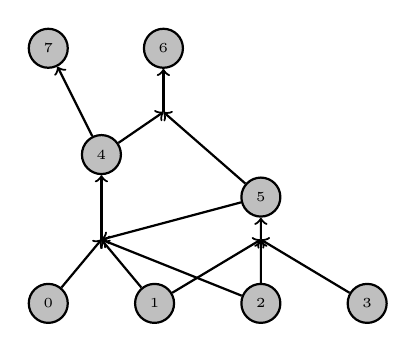
\begin{tikzpicture}[scale=0.45, yscale=1.2, thick] % , baseline = -3.5pt


	\node [circle, draw, thick, fill=gray!50] (T1) at (0,0) {\tiny $\lneuronof{0}$};
	\node [circle, draw, thick, fill=gray!50] (T2) at (3,0) {\tiny $\lneuronof{1}$};
	\node [circle, draw, thick, fill=gray!50] (T3) at (6,0) {\tiny $\lneuronof{2}$};
	\node [circle, draw, thick, fill=gray!50] (T4) at (9,0) {\tiny $\lneuronof{3}$};
	
	\node [circle, draw, thick, fill=gray!50] (ph) at (1.5,3.5) {\tiny $\lneuronof{4}$};
	\node [circle, draw, thick, fill=gray!50] (ph2) at (6,2.5) {\tiny  $\lneuronof{5}$};	
	
	\node [circle, draw, thick, fill=gray!50] (head) at (3.25,6) {\tiny $\lneuronof{6}$};
	\node [circle, draw, thick, fill=gray!50] (head2) at (0,6) {\tiny $\lneuronof{7}$};

	\draw[->] (ph) -- (head2);

	\coordinate (S3) at (3.25,4.5);
	\draw[->] (S3) -- (head);
	%\draw [->] (sel3) -- (S3);
	\draw [->] (ph2) -- (S3);
	\draw [->] (ph) -- (S3);
	
	\coordinate (S1) at (1.5,1.5);
	\draw[->] (S1) -- (ph);
	\draw [->] (T1) -- (S1);
	\draw [->] (T2) -- (S1);
	\draw [->] (T3) -- (S1);	
	\draw [->] (ph2) -- (S1);	
	
	\coordinate (S2) at (6,1.5);
	\draw[->] (S2) -- (ph2);
	%\draw [->] (sel) -- (S1);		
	%\draw [->] (sel2) -- (S2);

	\draw [->] (T2) -- (S2);
	\draw [->] (T3) -- (S2);	

	\draw [->] (T4) -- (S2);



\end{tikzpicture}
\end{center}
\caption{Example of an architecture graph $\graphof{\larchitecture}$ with input neurons $\inneuronset=\{\lneuronof{0},\lneuronof{1},\lneuronof{2},\lneuronof{3}\}$ and output neurons $\outneuronset=\{\lneuronof{6},\lneuronof{7}\}$
}
\label{fig:architectureGraph}
\end{figure}


\begin{theorem}
	Given fixed selection variables $\selvariableof{\larchitecture}$, the formula selecting neural network is the conjunction of output neurons, that is
	\begin{align*}
		\fsnnat{\catvariableof{\inneuronset},\selvariableof{\larchitecture}} = \bigwedge_{\lneuron\in\outneuronset} \lneuronat{\catvariableof{\inneuronset},\selvariableof{\larchitecture}} \, . 
	\end{align*}
\end{theorem}
\begin{proof}
	By effective calculus (see \theref{the:effectiveConjunction}), we have
		\[ \sbcontractionof{\rencodingofat{\land}{\catvariableof{\land},\shortcatvariables},\onehotmapofat{1}{\catvariableof{\land}}}{\shortcatvariables} = \bigotimes_{\catenumeratorin} \onehotmapofat{1}{\catvariableof{\catenumerator}} \]
	and thus
	\begin{align*}
		\fsnnat{\catvariableof{\inneuronset},\selvariableof{\larchitecture}}
		= \contractionof{
			\{\rencodingof{\lneuron} \, : \, \lneuron\in\nodesof{\larchitecture}/\inneuronset \} \cup \{\rencodingofat{\land}{\catvariableof{\land},\headvariableof{\lneuron}  \, : \, \lneuron\in\outneuronset}, \onehotmapofat{1}{\catvariableof{\land}}\}
		}{\catvariableof{\inneuronset},\selvariableof{\larchitecture}} \, . 
	\end{align*}
\end{proof}


% Combination of decompositions
By the commutation of contractions, we can further use \theref{the:neuronDecomposition} to decompose each tensor $\rencodingof{\lneuron}$ into connective and variable selecting components to get a sparse representation of a formula selecting neural network $\fsnn$.

%% Now as the definition!
%\begin{theorem}{Decomposition of formula selecting neural networks}\label{the:architectureDecomposition}
%	We have
%		\[ \rencodingof{\larchitecture} = \contractionof{\{\rencodingof{\lneuron} \, : \, \lneuron \in \larchitecture\}}{\catvariableof{\larchitecture},\shortcatvariables,\selvariableof{\larchitecture}} \]
%\end{theorem}
%\begin{proof}
%	By composition \theref{the:compositionByContraction}.
%	%\red{In addition: $X_{\larchitecture}$ specifying the headneurons! }
%\end{proof}

%% Now as the definition!
%% Relation between $\lneuron$ and $\rencodingof{\larchitecture}$
%Another useful property of encoded formula selecting architecture, is that we can retrieve any neuron by a simple contraction, as we show next.
%
%\begin{theorem}\label{the:formulaRetrieval}
%	Any neuron $\lneuron\in\larchitecture$ is retrieved by the contraction 
%		\[ \lneuron = \contractionof{\rencodingof{\larchitecture},\onehotmapof{1}[X_{\lneuron}]}{X\cup Z} \, . \]
%\end{theorem}
%\begin{proof}
%	First use the head neutralization property (Corollary~\ref{cor:onesHead}) in a parent stripping argument.
%	Then we are left with an architecture with $\lneuron$ being the only output neuron and use Corollary~\ref{cor:rhoToNormal} (we have $\restrictionofto{\mathrm{Id}}{[2]}=\onehotmapof{1}$).
%\end{proof}

% Alternative: Headneuron retrieval
%In case of multiple output neurons, the retrieval needs to be performed separately as in \theref{the:formulaRetrieval}, since contracting basis vectors $\onehotmapof{1}$ at multiple output neurons will retrieve the conjunction of those output neurons.




%\subsect{Skeleton Expressions}
%
%When only allowing for argument selections at the leaf level of the network, we get a skeleton expression.
%
%\begin{definition}\label{def:skeleton}
%	A skeleton expression
%		\[ \skeleton(\placeholderof{0},\ldots,\placeholderof{\selorder-1}) \]
%	is a composition of atom and connective selector maps, which are denoted by placeholders $\placeholderof{\selenumerator}$, where $\selenumerator\in[\selorder]$..
%	Each placeholder has a by $\selindexof{\selenumerator}$ enumerated list $\candidatelistof{\selenumerator}$ with cardinality $\seldimof{\selenumerator}= \cardof{\candidatelistof{\selenumerator}}$ of possible symbols denoting atoms or connectives to be placed in at this position.
%	This defines a map
%		\[ \skeleton : \left(\facstates\right) \times \left(\secfacstates\right) \rightarrow \{0,1\} \]
%	where $\skeleton(\atomindices,\selindices)$ denotes the formula given the selection of placeholders by $\selindices$, which is evaluated at the atoms $\atomindices$.
%\end{definition}

%\begin{definition}
%	A skeleton expression is a formula
%		\[ \skeleton(\placeholderof{0},\ldots,\placeholderof{\selorder-1}) \]
%	where instead of atoms and connectives there are placeholders $\placeholderof{\selenumerator}$, where $\selenumerator\in[\selorder]$.
%	Each skeleton has for each placeholder $\placeholderof{\selenumerator}$ a set $\candidatelistof{\selenumerator}$ of candidate atoms to be plugged in the placeholders.
%	We denote its cardinality to be $\seldimof{\selenumerator}= \cardof{\candidatelistof{\selenumerator}}$ and enumerate the elements $\placeholderof{\selenumerator}_{\selindexof{\selenumerator}}$ in each candidates list by an index $\selindexof{\selenumerator}\in[\seldimof{\selenumerator}]$.
%\end{definition}






%% ANOTHER EXAMPLE:





%\begin{definition}
%	Given a skeleton expression, the skeleton tensor is the map from the parameter space to the space of formula tensors, defined by
%	\begin{align}
%		 \skeletontensor : \rr^{\seldim} \rightarrow  \modelspace \quad , \quad
%		 \skeletontensor\left( \bigotimes_{\selenumeratorin}\unitvectoratof{\selenumerator}{\selindexof{\selenumerator}} \right) = \rencodingof{\skeletonof{\placeholderof{\selenumerator}_{\selindexof{\selenumerator}}\, : \, \selenumeratorin}}
%	\end{align}
%\end{definition}
%
%Using the canonical duality of tensors as maps and elements of tensor spaces, we can reinterpret is as a tensor \red{Domain representation of skeleton map}
%	\[ \skeletontensor \in \bigotimes_{\selenumerator\in[\selorder]} \rr^{\seldimof{\selenumerator}} \otimes  \modelspace  \, , \]
%which is the superposed formula tensor to a skeleton based parametrization.
%In the following, we investigate how to efficiently represent the skeleton tensor $\rencodingof{\skeleton}$ as a tensor network.









\sect{Application of Formula Selecting Networks}

There are two main applications of formula selecting networks.
First, when contracting the selection variables with a weight tensor we get a weighted sum of the parametrized formulas.
Second, when contracting the categorical variables with a distribution or a knowledge base, we get a tensor storing the satisfaction rates respectively the world counts of the parametrized formulas.

\subsect{Representation of selection encodings}

\red{In technical perspective: FSN provide efficient representation of $\sencodingof{\formulaset}$ 
-> Use for exponential families, structure learning.}

\begin{lemma}\label{lem:relToSelFSN}
	Given a set $\{\formulaof{\selindexlist} : \selindexlist\in\selstates\}$ of propositional formulas we define the statistic
		 \[ \formulaset : \catindices \rightarrow (\formulaof{\selindexlist}(\catindices))_{\selindexlist} \, . \]
	and the formula selecting map
		\[ \fselectionmap: \catindices , \selindexlist \rightarrow \formulaof{\selindexlist} (\catindices) \, . \]
	Then 
		\[ \sencodingofat{\formulaset}{\shortcatvariablelist, \shortselvariablelist} = \fselectionmap\left[\shortcatvariablelist, \shortselvariablelist \right] \, .  \]
		%\[ \sencodingofat{\formulaset}{\shortcatvariablelist, \shortselvariablelist}
		 %= \sbcontractionof{\rencodingofat{\fselectionmap}{\headvariableof{\fselectionmap}, \shortcatvariablelist, \shortselvariablelist}
		 %, \onehotmapofat{1}{\headvariableof{\fselectionmap}}}{\shortcatvariablelist, \shortselvariablelist} \, . \]
\end{lemma}
\begin{proof}
	For any indices $\shortselindices\in\selstates$ and $\shortcatindices\in\atomstates$ we have
	\begin{align*}
		\sencodingofat{\formulaset}{\shortcatvariablelist=\shortcatindices, \shortselvariablelist=\shortselindices}
		=  \formulaof{\selindexlist}(\catindices) =  \fselectionmap\left[\shortcatvariablelist=\shortcatindices, \shortselvariablelist=\shortselindices \right] \, . 
	\end{align*}
\end{proof}

%% Reason for relational encodings and selection encodings.
Technically, relational encodings have been exploited to derive decompositions based on basis calculus.
Selection encodings on the other hand enable the application of formula selecting networks as superpositions of formulas.



\subsect{Efficient Representation of Formulas}

\red{Weight contracted at the selection variables is elementary, then single formula retrieved.}

% Exponentially many formulas represented by linear demand
Formula Selecting Neural Networks are means to represent exponentially many formulas with linear (in sum of candidates list lengths) storage.
Their contraction with probability tensor networks, is thus a batchwise evaluation of exponentially many formulas.
This is possible due to redundancies in logical calculus due to modular combinations of subformulas.

% Retrieve functions
We can retrieve specific formulas by slicing the selection variables, i.e. for $\selindices$ we have
	\[ \exformula_{\selindices}[\shortcatvariables] = \fselectionmapat{\shortcatvariables,\selvariable=\selindices} \, .  \]

In a tensor network diagram we depict this by
\begin{center}
	\begin{tikzpicture}[thick, scale=0.35] % , baseline = -3.5pt

\node[anchor=east] (text) at (-3,0) {${\exformula_{\selindices}} \quad\quad {=}$};

\drawatomindices{0}{-4}
\draw (-1,3) rectangle (5, -3);
\node[anchor=center] (text) at (2,0) {$\bencodingof{\fselectionmap}$};

\draw[->] (2,3)--(2,5) node[midway,right] {\tiny $\headvariableof{\fselectionmap}$};
\draw (1,5) rectangle (3,7);
\node[anchor=center] (text) at (2,6) {$\tbasis$};

\draw[<-] (5,-2.25)--(7,-2.25) node[midway,below] {\tiny $\selvariableof{0}$}; 
\draw[<-] (5,-0.5)--(7,-0.5) node[midway,below] {\tiny $\selvariableof{1}$}; 
\node[anchor=center] (text) at (6,1) {$\vdots$};
\draw[<-] (5,2.25)--(7,2.25) node[midway,above] {\tiny $\selvariableof{\selorder\shortminus1}$};

\draw (7,1.5) rectangle (9,3);
\node[anchor=center] (text) at (8,2.25) {$\onehotmapof{\selindexof{\selorder\shortminus1}}$};

\draw (7,0.25) rectangle (9,-1.25);
\node[anchor=center] (text) at (8,-0.5) {$\onehotmapof{\selindexof{1}}$};

\draw (7,-1.5) rectangle (9,-3);
\node[anchor=center] (text) at (8,-2.25) {$\onehotmapof{\selindexof{0}}$};

\end{tikzpicture}
\end{center}

% Interpretation by dynamic programming
Another perspective on the efficient formula evaluation by selection tensor networks is dynamic computing.
Evaluating a formula requires evaluations of its subformulas, which are done by subcontractions and saved for different subformulas due to the additional selection legs.

% Storage problem of solutions
However, we need to avoid contracting the tensor with leaving all selection legs open, since this would require exponential storage demand.

% Sparse algorithm
We can avoid this storage bottleneck by extending the contractions by additional cores leaving less variable legs open.
This is the case when contracting gradients of the parameter tensor networks in alternating least squares approaches.
Other methods avoiding the bottleneck can be constructed by MCMC sampling, for example Gibbs Sampling.
Here we only need to vary local components of the formula reflected in keeping only single variable legs open.



\subsect{Batch contraction of parametrized formulas}

Given a set $\formulaset$ of formulas, we build a formula selecting network parametrizing the formulas.
The contraction 
\begin{align*}
	\contractionof{\extnet,\fselectionmap}{\shortselvariables} 
\end{align*}
is a tensor containing the contractions of the formulas $\formulaof{\shortselindices}$ with an arbitrary tensor network $\extnet$ as
\begin{align*}
	\sbcontraction{\extnet,\formulaof{\shortselindices}} = \sbcontractionof{\extnet,\fselectionmap}{\shortselvariables=\shortselindices} \, . 
\end{align*}


\subsect{Average contraction of parametrized formulas}

We show in the next two examples, how a full contraction of the formula selecting map with a probability distribution or a knowledge base can be interpreted.

\begin{example}[Average satisfaction of formulas]
	The average of the formula satisfactions in $\formulaset$ giben a probability tensor $\probtensor$ is 
		\[ \frac{1}{\prod_{\selenumeratorin}\seldimof{\selenumerator}} \cdot \sbcontraction{\probtensor,\sencodingof{\formulaset}} \, . \]
\end{example}


\begin{example}[Deciding whether any formula is not contradicted]
	For example: We want to decide, whether there is a formula in $\formulaset$ not contradicted by a Knowledge base $\kb$.
	This is the case if and only if 
		\[ \sbcontraction{\kb,\sencodingof{\formulaset}} = 0 \, .  \]
	We use \lemref{lem:relToSelFSN} to get that $\sencodingof{\formulaset}=\fselectionmap$.
	When the formulas are representable in a folded scheme, we find tensor network decompositions of $\fselectionmap$ and exploit them along efficient representations of $\kb$ in an efficient calculation of $\sbcontraction{\kb,\sencodingof{\formulaset}} $.
	This is further equal to 
		\[ \kb \models \lnot \left( \bigvee_{\exformula\in\formulaset} \exformula\right) \, . \]
\end{example}



%\subsect{Neuro-Symbolic Architectures}
%
%%% Neuro-Symbolic Architecture
%We understand selector tensor networks as a neuro-symbolic architecture, where the selector variables are understood as parameters and the processed variables as neural activation variables.
%The orientation of the tensor network organizes the variables in layers.




\sect{Examples of formula selecting neural networks}

%Here we provide examples of exponential families
%\red{See further: \charef{cha:energyRepresentation} studying the exact representation of energy as a weighted superposition of formulas.}

%\subsect{Boltzmann Machines}
%The inverse is the representation of a given distribution by a Boltzmann machine?


\subsect{Correlation}


For example (see Figure \ref{fig:AndSupFTDecomposition}) consider the logical neuron with single activation candidate $\{\land\}$ and two variable selectors selecting $\catorder$ atomic variables $\shortcatvariables$.
The expressivity of this network is the set of all conjunctions of the atoms
	\[ \{\catvariableof{\atomenumerator} \land \catvariableof{\secatomenumerator} \, : \, \atomenumerator,\secatomenumerator\in[\atomorder] \} \]


% Covariance measure
Contracting with a probability distribution, we use the tensor
	\[ \hypercoreat{\selvariableof{\vselectionsymbol,0},\selvariableof{\vselectionsymbol,1}} = \sbcontractionof{\fsnn}{\selvariableof{\vselectionsymbol,0},\selvariableof{\vselectionsymbol,1}} \]
to read of covariances as
	\[ \mathrm{Cov}(\catvariableof{\atomenumerator},\catvariableof{\secatomenumerator}) = \hypercoreat{\selvariableof{\vselectionsymbol,0}=\atomenumerator,\selvariableof{\vselectionsymbol,1}=\secatomenumerator}  - 
	\hypercoreat{\selvariableof{\vselectionsymbol,0}=\atomenumerator,\selvariableof{\vselectionsymbol,1}=\atomenumerator}  \cdot \hypercoreat{\selvariableof{\vselectionsymbol,0}=\secatomenumerator,\selvariableof{\vselectionsymbol,1}=\secatomenumerator} \, .  \]
	
	
	

%	\[ \skeleton = \placeholderof{1} \land \placeholderof{2} \]
%with the candidates for each placeholder being a set of $\atomorder$ atoms.

\begin{figure}[h]
\begin{center}
	\begin{tikzpicture}[thick, scale=0.35] % , baseline = -3.5pt

\drawatomindices{0}{-4}
\draw (-1,-1) rectangle (5, -3);
\node[anchor=center] (text) at (2,-2) {$\bencodingof{\atomicformulaof{\selindexof{1}} \land \atomicformulaof{\selindexof{2}}}$};

\draw[->] (2,-1)--(2,1) node[midway,right] {\tiny ${\headvariableof{\selindexof{1}} \land \headvariableof{\selindexof{2}}}$};

\draw[<-] (5,-2.5)--(7,-2.5) node[midway,below] {\tiny $\selvariable_{1}$};
\draw[<-] (5,-1.5)--(7,-1.5) node[midway,above] {\tiny $\selvariable_{0}$};

\draw (7,-1) rectangle (9, -3);
\node[anchor=center] (text) at (8,-2) {$\canparam$};


		
\node[anchor=center] (text) at (12,-2) {${=}$};


\begin{scope}[shift={(17,8)}]
	\begin{scope}[shift={(0,-10)}]

		\draw[->] (5.5,5) -- (5.5,7) node[midway, right] {\tiny ${\headvariableof{\selindexof{1}} \land \headvariableof{\selindexof{2}}}$};
		\draw (1,3) rectangle (10, 5);
		\node[anchor=center] (text) at (5.5,4) {$\bencodingof{\land}$};

			
		% SelectorCores
		\draw[->] (2,1) -- (2,3) node[midway, left] {\tiny ${\headvariableof{\selindexof{2}}}$};
		\draw (-1,1) rectangle (5, -1);
		\node[anchor=center] (text) at (2,0) {$\selectorcoreof{2}$};
		\draw (5,0) -- (12,0);
		\draw[<-] (12,0) -- (14,0) node[midway, above] {\tiny $\selvariable_{1}$};
		\begin{scope}[shift={(0,-2)}]
			\draw[<-] (0,1)--(0,-3) node[midway,left] {\tiny $\catvariableof{0}$}; 
			\draw[<-] (1.5,1)--(1.5,-3) node[midway,left] {\tiny $\catvariableof{1}$}; 
			\node[anchor=center] (text) at (3,0) {$\cdots$};
			\draw[<-] (4,1)--(4,-3) node[midway,right] {\tiny $\catvariableof{\atomorder\shortminus1}$}; 
		\end{scope}


		\draw (9,-1) -- (9,1);
		\draw[->] (9,1) -- (9,3) node[midway, left] {\tiny ${\headvariableof{\selindexof{1}}}$};
		\draw (6,-3) rectangle (12, -1);
		\node[anchor=center] (text) at (9,-2) {$\selectorcoreof{1}$};
		\draw[<-] (12,-2) -- (14,-2) node[midway, above] {\tiny $\selvariable_{0}$};
		\drawatomindices{7}{-4}	
		
		% ParameterCores
		\draw (14,1) rectangle (16, -3);
		\node[anchor=center] (text) at (15,-1) {$\canparam$};
		
		\begin{scope}[shift={(-3.5,8)}]
			\draw[fill] (7.5,-15) circle (0.15cm);
			\draw[] (7.5,-15) to[bend left=25] (3.5,-13);
			\draw[] (7.5,-15) to[bend right=25] (10.5,-13);

			\draw[fill] (9,-15.25) circle (0.15cm);
			\draw[] (9,-15.25) to[bend left=25] (5,-13);
			\draw[] (9,-15.25) to[bend right=25] (12,-13);

			\draw[fill] (11.5,-15) circle (0.15cm);
			\draw[] (11.5,-15) to[bend left=25] (7.5,-13);
			\draw[] (11.5,-15) to[bend right=25] (14.5,-13);

			\drawatomindices{7.5}{-16}

		\end{scope}

	\end{scope}
\end{scope}

\end{tikzpicture}
\end{center}
\caption{Superposition of the encoded formulas $\rencodingof{\atomicformulaof{\selindexof{1}} \land \atomicformulaof{\selindexof{2}}}$ with weight $\canparam_{\selindexof{1} \selindexof{2}}$}
\label{fig:AndSupFTDecomposition}
\end{figure}



\subsect{Conjunctive and Disjunctive Normal Forms}%\label{sec:CNFasFormulaSelection}

% Architecture
We can represent any propositional knowledge base by the following scheme:
Literal selecting neurons by connective identity/negation (selecting positive/negative literal) and selecting one of the atoms.
Single output neuron representing the disjunction combining the literal selecting neurons.
Number of neurons defined by the maximal clause size plus one.
Smaller clauses can be covered when adding False as a possible choice (The respective neuron has to choose the identity, otherwise the full clause will be trivial).

% Parameter
The parameter core is in the basis CP format and each slice selects a clause of the knowledge base.
When taking the slice values to infinity (e.g. by an annealing procedure), the represented member of the exponential family converges to the uniform distribution of the models of the knowledge base.


\red{Useful to derive basis+ CP format based on CNF!}


% Representation by selection tensor networks
\begin{remark}[Minterms and Maxterms]
	All minterms and maxterms can be represented by a two layer selection tensor networks without variable selection in two layers.
	The bottom layer has an $\lnot/\mathrm{Id}$ connective selection neuron to each atom and the upper layer consists of a single $\atomorder$ary conjunction.
\end{remark}




\sect{Extension to variables of larger dimension}

Connective selecting tensors: Can encode arbitrary functions $h_{\selindex}$ of discrete variables, but need $\catvariableof{\cselectionmap}$ to be an enumeration of the states, in particular to be of dimension
	\[ \catdimof{\cselectionmap} = \cardof{ \cup_{\selindexin} \imageof{h_{\selindex}} } \, . \]
	
Variable selecting tensors can be understood as specific cases of connective selecting tensors and can thus also be generalized in a straight forward manner by
	\[ \catdimof{\cselectionmap} = \cardof{ \cup_{\selindexin} \imageof{h_{\selindex}} } \, .  \]
	
State selecting tensors are directly 


\begin{example}[Discretization of a continuous neuron]
	Let there be a neuron
		\[ \sigma( w, y) : \rr \times \rr^{\catorder} \rightarrow \rr \, .\]
	When $w \in \arbsetof{weight}\subset \rr^{\catorder}$ and $x \in \arbsetof{x}\subset \rr^{\catorder}$ have
		\[ \cardof{\sigma( \contractionof{w, x} )} \leq \cardof{\arbsetof{weight}} \cdot \cardof{\arbsetof{x}} \, . \] 

	To represent the discretization of the neuron, we use the subset encoding scheme of \defref{def:subsetEncoding}.
	The variables $\indvariableof{weight}$ indexing $\arbsetof{weight}$ will be understood as selection incoming variables and the variables $\indvariableof{weight}$ indexing $\arbsetof{weight}$ as categorical incoming variables.
	We further define a variable $\indvariableof{\sigma}$ indexing $\imageof{\restrictionofto{\sigma}{\arbsetof{weight}\times\arbsetof{x}}}$ and have a tensor
		\[ \rencodingofat{\sigma}{\indvariableof{\sigma},\indvariableof{\arbsetof{x}},\indvariableof{weight}} \, . \] 

	If the neuron is of the form
		\[ \sigma(w,x) = \psi(\sum_i w_i \cdot x_i)\]
	a decomposition into multiplication at each coordinate and summation of the results, with relational encodings for each, can be done.
\end{example}
